\newpage
\section{Context-free Language}
Context-free Grammar

e.g. 
\begin{itemize}
    \item start symbol: $S$
    \item rule: $S \to aSb$, $S\to A$, $A\to c$, $A\to e$
    \begin{itemize}
        \item non-terminal: $S, A$
        \item terminal: $a,b,c$
    \end{itemize}
\end{itemize}

\subsection{Definition}

\begin{definition}
    A content-free grammar $G=(V,\Sigma, S, R)$,
    \begin{itemize}
        \item $V$ a \textbf{finite} set of symbols
        \item $\Sigma\subseteq V$: the set of terminals
        \subitem $V-\Sigma$: the set of non-terminals
        \item $S\in V-\Sigma$: start symbol
        \item $R\subseteq (V-\Sigma)\times V^*$: a \textbf{finite} set of rules
    \end{itemize}
\end{definition}

\begin{definition}[derive in one step]
    $\forall x,y,u \in V^*$, $\forall A\in V-\Sigma$,
    \begin{align*}
        xAy\Rightarrow_G xuy \text{ if } (A,u)\in R
    \end{align*}
\end{definition}

\begin{definition}[a derivation from $w$ to $u$]
    $\forall w,u \in V^*$,
    \begin{align*}
        w\Rightarrow_G^*u \text{ if } w=u\text{ or }w\Rightarrow_G \dots \Rightarrow_G u
    \end{align*}
\end{definition}

\begin{definition}
    $G$ generates $w\in \Sigma^*$ if $S\Rightarrow_G^* w$. 
    \begin{align*}
        L(G)=\{ w\in \Sigma^*: G\text{ generates }w \}
    \end{align*}
    $G$ generates $L(G)$, called content-free language
\end{definition}

e.g. Show that $\{ w\in \{ a,b \}^*: w=w^R \}$ (回文串) is content-free.\\
$S\to e|a|b|aSa|bSb$. 

need to proof:
\begin{itemize}
    \item if $w\in L(G)$, $w=w^R$. (归纳 $w$ 替换的次数)
    \item if $w=w^R$, $w\in L(G)$. (归纳 $|w|$)
\end{itemize}

e.g. have $S\to SS$, $S\to (S)$, $S\to e$, generates $()()$. 
\begin{itemize}
    \item $S\Rightarrow SS\Rightarrow (S)S\Rightarrow ()S\Rightarrow()(S)\Rightarrow()()$ (leftmost derivation)
    \item $S\Rightarrow SS\Rightarrow S(S)\Rightarrow S()\Rightarrow (S)()\Rightarrow ()()$(rightmost derivation)
\end{itemize}
parse tree is same. 

\begin{definition}[parse tree]
    \quad

    \begin{itemize}
        \item internal node: non-terminal
        \item leaves: terminal or $e$, $e$ must be the only child of its parent
        \item edge: $A\to a_1,\dots,a_n$
        
        \begin{figure}[H]
            \centering
            \begin{tikzpicture}
                \node {$A$}
                    child {node {$a_1$}}
                    child {node {$\dots$}}
                    child {node {$a_n$}};
            \end{tikzpicture}    
        \end{figure}

        \item the yield of parse tree: e.g. $a_1,a_n$
    \end{itemize}
\end{definition}

e.g. 
\begin{itemize}
    \item $E\to E+E$, 
    \item $E\to E\times E$, 
    \item $E\to a$
\end{itemize}
\begin{figure}[!htb]
    \centering
    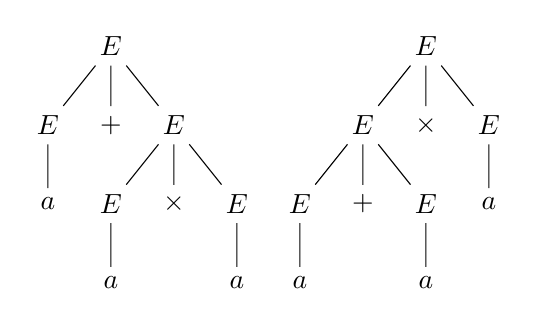
\begin{tikzpicture}[sibling distance = 0.8cm, level distance = 1cm]
        \node at (-2,0) {$E$}
            child{node{$E$}
                child{node{$a$}}
            }
            child{node{$+$}}
            child{node{$E$}
                child{node{$E$}
                    child{node{$a$}}
                }
                child{node{$\times$}}
                child{node{$E$}
                    child{node{$a$}}
                }
            }
        ;
        \node at (2,0) {$E$}
            child{node{$E$}
                child{node{$E$}
                    child{node{$a$}}
                }
                child{node{$+$}}
                child{node{$E$}
                    child{node{$a$}}
                }
            }
            child{node{$\times$}}
            child{node{$E$}
                child{node{$a$}}
            }
        ;
    \end{tikzpicture}
    % \caption{}
\end{figure}


ambiguous

but 
\begin{itemize}
    \item $E\to E+T$, 
    \item $E\to T$, 
    \item $T\to T \times F$, 
    \item $T\to F$, 
    \item $F\to (E)$, 
    \item $F\to a$
\end{itemize}

no ambiguous

\begin{figure}[!htb]
    \centering
    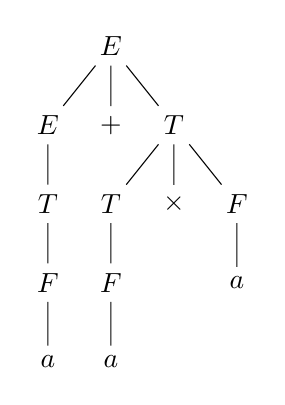
\begin{tikzpicture}[sibling distance = 0.8cm, level distance = 1cm]
        \node{$E$}
            child{node{$E$}
                child{node{$T$}
                    child{node{$F$}
                        child{node{$a$}}
                    }
                }
            }
            child{node{$+$}}
            child{node{$T$}
                child{node{$T$}
                    child{node{$F$}
                        child{node{$a$}}
                    }
                }
                child{node{$\times$}}
                child{node{$F$}
                    child{node{$a$}}
                }
            }
        ;
    \end{tikzpicture}
    % \caption{}
\end{figure}


Fact: $\{ a^ib^jc^k:i=j \text{ or }j=k \}$ inherently language (任意生成此 的 language 都有歧义) 

\subsection{Chomsky nrom form (CNF)}

\begin{definition}
    A CFG is in Chomsky nrom form (CNF) if every rule is of one of the following forms:
    \begin{enumerate}
        \item $S\to e$
        \item $A\to BC$, $B,C\in V-\Sigma-\{S\}$
        \item $A\to a$, $a\in \Sigma$
    \end{enumerate}
\end{definition}

Observation: Suppose that $G$ is a CFG in CNF. If $G$ generates a string of length $n\ge 1$, \# length if derivation is $2n-1$. 

\begin{theorem}
    Every CFG has an equivalent CFG in CNF
\end{theorem}
sketch of proof: 不满足的几种情况
\begin{enumerate}
    \item $S$ appears on the right side of a rule
    \subitem solution: create new start symbol $S_0$, let $S_0\to S$
    \item $A\to e$ for $A\ne S$
    \subitem solution: e.g. $A\to e$, $B\to ACA$, delete $A\to e$, add $B\to AC$, $B\to CA$, $B\to C$. 所有类似的规则作类似的处理. 
    \item $A\to B$, for some $B\in V-\Sigma$
    \subitem solution: If $A\ne S$, the same as $A\to e$. If $A=S$: e.g. $S\to B$, $B\to AC$, $B\to CD$, delete all, add $S\to AC$, $S\to CD$
    \item $A\to u_1,\dots,u_k$, $k\ge 3, u_i \in V$
    \subitem solution: delete it, add $A\to u_1V_2$, $V_2\to u_2,\dots,u_k$ and so on. 
    \item $A\to u_1 u_2$, at least one $u_i \in \Sigma$
    \subitem solution: e.g. $A\to bC$, delete it, add $A\to BC$, $B\to b$
\end{enumerate}

\subsection{Pushdown Automata(PDA)}
PDA $\iff$ CFG. PDA = NFA + stack

have input tape, state control, stack

\begin{definition}[Pushdown Automata]
    A PDA is a 6-tuple $P=(K, \Gamma, \Sigma, \Delta, s, F)$
    \begin{itemize}
        \item $\Gamma$: stack alphabet
        \item $\Delta$: transition relation: a \textbf{finite} subset of 
        \begin{align*}
            (K\times (\Sigma\cup \{ e \})\times\Gamma^*)\times(K\times\Gamma^*)
        \end{align*}
        \begin{itemize}
            \item 1st $K$: current state
            \item $\Sigma\cup \{ e \}$: current symbol that is read
            \item 1st $\Gamma^*$: pop string at the top of stack
            \item 2nd $K$: next state
            \item 2nd $\Gamma^*$: push a string onto the stack
        \end{itemize}
    \end{itemize}
\end{definition}

e.g. $((p,a,123),(q,45))$, 在状态$p$时, 若读到$a$, 且stack顶有 123, 将 123 pop, 然后压入 45, 状态$p\to q$. $((p,a,e),(q,B))$, 这个 stack 一直满足条件, 顶一定有 $e$. 

\begin{definition}
    A configuration of $P$ is a member of $K\times \Sigma^*\times \Gamma^*$
    \begin{itemize}
        \item current state
        \item unread input
        \item stack control
    \end{itemize}
\end{definition}

\begin{definition}
    $(p,x,\alpha)\vdash_P (q,y,\beta)$ if $\exists ((p,a,r), (q,\eta ))\in \Delta$ s.t. 
    \begin{align*}
        x&=ay\\
        \alpha&=r\tau \text{ and }\beta = \eta \tau 
    \end{align*}
    for some $\tau \in \Gamma^*$
\end{definition}

\begin{definition}
    $(p,x,\alpha)\vdash_P^* (q,y,\beta)$ if $(p,x,\alpha)=(q,y,\beta)$ or $(p,x,\alpha)\vdash_P\cdots\vdash_P(q,y,\beta)$
\end{definition}

\begin{definition}
    $P$ accepts $w\in\Sigma^*$ if
    \begin{align*}
        (s,w,e)\vdash_P^*(q,e,e)
    \end{align*}
    for some $q\in\Gamma$
    \begin{enumerate}
        \item finial state
        \item consume all the input
        \item empty stack
    \end{enumerate}
\end{definition}

\begin{definition}
    $L(P)=\{ w\in\Sigma^*: P\text{ accepts }w \}$. $P$ accepts $L(P)$
\end{definition}

e.g. $\{ w\in \{ 0,1 \}^*: \text{\# 0's = \# 1's in } w\}$ 设计 PDA, accepts it. 
\begin{itemize}
    \item $K=\{ s\}$
    \item $F=\{ s\}$
    \item $\Sigma=\{ 0,1 \}$
    \item $\Gamma=\{ 0,1 \}$
    \begin{align*}
        \Delta=\{&((s,0,1), (s,e))\\
        &((s,0,e),(s,0))\\
        &((s,1,0), (s,e))\\
        &((s,1,e),(s,1))
         \}
    \end{align*}
\end{itemize}
PDA 是非确定的, 也有猜的能力. 

CFG $\iff$ PDA

CFG $\to$ PDA

Idea:
\begin{enumerate}
    \item in stack, non-deterministic generates a string from $S$
    \item compute it to the input 
    \item accepts if they match
\end{enumerate}
\begin{figure}[!htb]
    \centering
    \begin{tikzpicture}
        \coordinate (stack1) at (0,2);
        \coordinate (stack2) at (0,0);
        \coordinate (stack3) at (0.5,0);
        \coordinate (stack4) at (0.5,2);

        \foreach \x in {0,...,5}{
            \coordinate (o) at (1.5*\x,0);
            \draw ($(o)+(stack1)$)--($(o)+(stack2)$)--($(o)+(stack3)$)--($(o)+(stack4)$);
        }

        \foreach \x in {0,...,4}{
            \coordinate (o) at (1.5*\x + 0.6,1);
            % \node at (o) {$S$};
            \draw [->] (o)--($(o)+(0.8,0)$);
        }

        %0
        \coordinate (ls) at (1.5*0,0.4*1);
        \draw (ls)--($(ls)+(0.5,0)$);
        \node at ($(ls)+(0.25, -0.2)$) {$S$};
        %1
        \coordinate (ls) at (1.5*1,0.4*1);
        \draw (ls)--($(ls)+(0.5,0)$);
        \node at ($(ls)+(0.25, -0.2)$) {$b$};
        \coordinate (ls) at (1.5*1,0.4*2);
        \draw (ls)--($(ls)+(0.5,0)$);
        \node at ($(ls)+(0.25, -0.2)$) {$S$};
        \coordinate (ls) at (1.5*1,0.4*3);
        \draw (ls)--($(ls)+(0.5,0)$);
        \node at ($(ls)+(0.25, -0.2)$) {$a$};
        %2
        \coordinate (ls) at (1.5*2,0.4*1);
        \draw (ls)--($(ls)+(0.5,0)$);
        \node at ($(ls)+(0.25, -0.2)$) {$b$};
        \coordinate (ls) at (1.5*2,0.4*2);
        \draw (ls)--($(ls)+(0.5,0)$);
        \node at ($(ls)+(0.25, -0.2)$) {$S$};
        %3
        \coordinate (ls) at (1.5*3,0.4*1);
        \draw (ls)--($(ls)+(0.5,0)$);
        \node at ($(ls)+(0.25, -0.2)$) {$b$};
        \coordinate (ls) at (1.5*3,0.4*2);
        \draw (ls)--($(ls)+(0.5,0)$);
        \node at ($(ls)+(0.25, -0.2)$) {$b$};
        \coordinate (ls) at (1.5*3,0.4*3);
        \draw (ls)--($(ls)+(0.5,0)$);
        \node at ($(ls)+(0.25, -0.2)$) {$S$};
        \coordinate (ls) at (1.5*3,0.4*4);
        \draw (ls)--($(ls)+(0.5,0)$);
        \node at ($(ls)+(0.25, -0.2)$) {$a$};
        %4
        \coordinate (ls) at (1.5*4,0.4*1);
        \draw (ls)--($(ls)+(0.5,0)$);
        \node at ($(ls)+(0.25, -0.2)$) {$b$};
        \coordinate (ls) at (1.5*4,0.4*2);
        \draw (ls)--($(ls)+(0.5,0)$);
        \node at ($(ls)+(0.25, -0.2)$) {$b$};
        \coordinate (ls) at (1.5*4,0.4*3);
        \draw (ls)--($(ls)+(0.5,0)$);
        \node at ($(ls)+(0.25, -0.2)$) {$S$};
        %5
        \coordinate (ls) at (1.5*5,0.4*1);
        \draw (ls)--($(ls)+(0.5,0)$);
        \node at ($(ls)+(0.25, -0.2)$) {$b$};
        \coordinate (ls) at (1.5*5,0.4*2);
        \draw (ls)--($(ls)+(0.5,0)$);
        \node at ($(ls)+(0.25, -0.2)$) {$b$};
    \end{tikzpicture}
    \caption{Idea of CFG $\to$ PDA. e.g. $S\to aSb|e$, aabb}
\end{figure}


\begin{proof}
    CFG $\to$ PDA

    $G=(V,\Sigma, S,R)\to M=(K,\Sigma, \Gamma, \Delta, s, F) \iff L(M)=L(G)$
    \begin{itemize}
        \item $\Gamma=V$
        \item $K=\{ s,f \}$
        \item $F=\{ f \}$
        \item 
        \begin{align*}
            \Delta=\{ &((s,e,e),(f,S)),\\
            &((f,e,A),(f,u))\text{ for each }(A,u)\in R,\\
            &((f,a,a),(f,e))\text{ for each } a\in\Sigma\}
        \end{align*}
    \end{itemize}
\end{proof}

PDA $\to$ simple PDA $\to$ CFG 

\begin{definition}
    A PDA $M=(K,\Sigma, \Gamma, \Delta, s,F)$ is simple if 
    \begin{enumerate}
        \item $|F|=1$
        \item for each transition $((p,a,\alpha),(q,\beta))\in\Delta$ 
        \subitem either $\alpha=e$ and $|\beta|=1$ 
        \subitem or $|\alpha|=1$ and $\beta=e$
    \end{enumerate}
\end{definition}

PDA $\to$ simple PDA
\begin{enumerate}
    \item If $|F|>1$, create a new state $f'$, for each $q\in F$, add a new transition $((q,e,e),(f',e))$, $F:=\{ f' \}$. 
    \item only four cases, as $((p,a,\alpha),(q,\beta))$
    \begin{enumerate}
        \item $|\alpha|\ge 1$ and $|\beta|\ge 1$
        \subitem create a new state $r$, replace the transition with 
        \begin{align*}
            ((p,a,\alpha),&(r,e))\\
            ((r,e,e),&(q,\beta))
        \end{align*}
        \item $|\alpha|>1$ and $\beta=e$
        \subitem $\alpha=c_1,c_2,\dots,c_k$, create new state $r_1,\dots,r_{k-1}$. replace the transition with 
        \begin{align*}
            ((p,a,c_1),&(r_1,e))\\
            ((r_1,e,c_2),&(r_2,e))\\
            \vdots&\\
            ((r_{k-1},e,c_k),&(q,e))
        \end{align*}
        \item $\alpha=e$ and $|\beta|>1$
        \subitem same as 2
        \item $\alpha=e$ and $\beta=e$
        \subitem create a new state $r$, pick a $b$ from $\Gamma$,
        \begin{align*}
            ((p,a,e),&(r,b))\\
            ((r,e,b),&(q,e))
        \end{align*}
    \end{enumerate}
\end{enumerate}

simple PDA $\to$ CFG

a simple PDA $P=(K,\Sigma, \Gamma,\Delta,s,F)$ $\to$ $G=(V,\Sigma, S,R)$

\begin{itemize}
    \item non-terminal: $\{ A_{pq}: \text{ for }p,q\in K \}$
    \subitem Goal: 
    \begin{align*}
        &A_{pq}\to w\in\Sigma^*\\
        \iff& w\in \{ w\in\Sigma^*:(p,u,e)\vdash^*_p(q,e,e) \}
    \end{align*}
    \item $S=A_{sf}$, $F=\{ f \}$(simple)
    \item $R=$
    \begin{enumerate}
        \item $\forall p\in K$, $A_{pp}\to e$
        \item $\forall p,q\in K$,
        \subitem $A_{pq}\to A_{pr}A_{rq}$ $\forall r\in K$
        \subitem $A_{pq}\to aA_{p'q'}b$ \\
        $\forall ((p,a,e),(p',\alpha))\in\Delta$ and $((q',b,\alpha),(q,e))\in\Delta$ for some $\alpha\in\Gamma$
    \end{enumerate}
\end{itemize}

proof idea: 
\begin{itemize}
    \item $\Rightarrow$ by induction on length of derivation from $A_{pq}$ to $w$
    \item $\Leftarrow$ by induction on \# steps of computation. 
\end{itemize}

PDA $\to$ define CFG

\begin{theorem}
    Every regular language is content-free. 
\end{theorem}

\subsection{CFL properties}
CFG closure properties: $\cup,\circ,*$ is closure, $\cap,\bar{A}$ isn't closure. 

$G_A=(V_A,\Sigma_A,S_A,R_A)$, $G_B=(V_B,\Sigma_B,S_B,R_B)$
\begin{itemize}
    \item $G_{A\cup B}$: $S\to S_A | S_B$
    \item $G_{A\circ B}$: $S\to S_AS_B$
    \item $G_{A^*}$: $S\to e|SS_A$
\end{itemize}

$A=\{ a^ib^jc^k:i=j \}, B=\{ a^ib^jc^k : j=k\} \to $ $A$ and $B$ are content-free. 
\begin{itemize}
    \item $A\cap B=\{ a^nb^nc^n:n\ge 0 \}$ not content-free.
    \item $A\cap B=\overline{\bar{A}\cup \bar{B}}$ not content-free.
\end{itemize}
so CFL is not closed under $\cap$ or $\bar{A}$

\begin{theorem}[Pumping theorem for CFL]
    Let $L$ be a content-free language. There exists an integer $p>0$ such that any $w\in L$ with $|w|\ge p$ can be divided into $w=uvxyz$ satifiying:
    \begin{enumerate}
        \item $uv^ixy^iz\in L$ for any $i\ge 0$
        \item $|v|+|y|>0$
        \item $|vxy|\le p$
    \end{enumerate}
\end{theorem}

e.g. $\{ a^n b^n:n\ge 0 \}, p=2$, $u=x=z=e, v=a, y=b$ 

\begin{figure}[!htb]
    \centering
    \begin{tikzpicture}
        \draw (0,0)--(6,0)--(3,4)--cycle;

        
        \coordinate (Q1) at (3,1.2);
        \draw [dashed] (3,4)--(Q1);
        \draw [dashed] (Q1)--(2.4,0);
        \draw [dashed] (Q1)--(3.6,0);

        \coordinate (Q2) at (3,2.4);
        \draw [dashed] (3,4)--(Q2);
        \draw [dashed] (Q2)--(1.2,0);
        \draw [dashed] (Q2)--(4.8,0);

        \node at (3,4.2) {$S$};
        \node at ($(Q1)+(0.2,0)$) {$Q$};
        \node at ($(Q2)+(0.2,0)$) {$Q$};

        \node at (1.2*0+0.6, -0.2) {$u$};
        \node at (1.2*1+0.6, -0.2) {$v$};
        \node at (1.2*2+0.6, -0.2) {$x$};
        \node at (1.2*3+0.6, -0.2) {$y$};
        \node at (1.2*4+0.6, -0.2) {$z$};
    \end{tikzpicture}
    \caption{Idea's parse tree}
    \label{fig:ppt}
\end{figure}

non-terminal $|V-\Sigma|$ finite. $Q$ exists twice in a long enough path, draw $Q$ subtree. 
\begin{itemize}
    \item $S\Rightarrow^*uQz$
    \item $Q\Rightarrow^*vQy$
    \item $Q\Rightarrow^*x$
\end{itemize}
$S\Rightarrow^*uv^ixy^iz\in L$, $\forall i\ge 0$. 

\begin{proof}
    $L$ is content-free $\Rightarrow$ $\exists G=(V,\Sigma, S,R)$ with $L(G)=L$. 

    Let $b=\max\{ |u|: (A,u)\in R \}$, fanout $\le b$

    Fact: If a tree with famout $\le b$ has $n$ leaves, its height(\# edges on the longest descending path) $\ge \log_b n$. 

    $p=b^{|V-\Sigma|+1}$, $w\in L$ with $|w|\ge p$. Let $T$ be the parse tree of $w$, (with smallest \# nodes), height of $T\ge \log_b p=|V-\Sigma|+1$. 
    \begin{itemize}
        \item \# edges $\ge |V-\Sigma|+1$, 
        \item \# nodes $\ge |V-\Sigma|+2$, 
        \item \# non-terminal on the path $\ge |V-\Sigma|+1$
    \end{itemize}
    some non-terminal $Q$ appears twice on the path, as shwon in \textbf{Figure} \ref{fig:ppt}. 
    \begin{enumerate}
        \item $uv^ixy^iz\in L$ for any $i\ge 0$ 显然
        \item $|u|+|y|>0$
        \subitem If $v=y=e, w=uxz$, parse tree smaller than $T$, but $T$ is the smallest, contradiction. 
        \begin{figure}[!htb]
            \centering
            \begin{tikzpicture}
                % \draw (0,0)--(6,0)--(3,4)--cycle;
                \draw (1.2,0)--(0,0)--(3,4)--(6,0)--(4.8,0);
        
                \coordinate (Q2) at (3,2.4);
                \draw [dashed] (3,4)--(Q2);
                \draw [dashed] (Q2)--(1.2,0);
                \draw [dashed] (Q2)--(4.8,0);

                \draw (2.4, 1.6)--(3.6, 1.6);
        
                \node at (3,4.2) {$S$};
                \node at ($(Q2)+(0.2,0)$) {$Q$};
        
                \node at (1.2*0+0.6, -0.2) {$u$};
                \node at (1.2*4+0.6, -0.2) {$z$};
                \node at (3, 1.4) {$x$};
            \end{tikzpicture}
            \caption{2)'s parse tree}
        \end{figure}
        \item $|vxy|\le p$ 
        \begin{figure}[!htb]
            \centering
            \begin{tikzpicture}
                \draw (1.2,0)--(Q2)--(4.8,0)--cycle;
        
                \coordinate (Q2) at (3,2.4);
                \coordinate (Q1) at (3,1.2);
                \coordinate (a) at (3.2, 0);
                \draw [dashed] (Q2)--(Q1);
                \draw [dashed] (Q1)--(2.4,0);
                \draw [dashed] (Q1)--(3.6,0);
                \draw [dashed] (Q1)--(a);
                \node at ($(Q1)+(0.2,0)$) {$Q$};
                \node at ($(Q2)+(0.2,0)$) {$Q$};

                \node at ($(a)+(-0.2,0.2)$) {$a$};

                \node at (1.2*1+0.6, -0.2) {$v$};
                \node at (1.2*2+0.6, -0.2) {$x$};
                \node at (1.2*3+0.6, -0.2) {$y$};
            \end{tikzpicture}
            \caption{3)'s parse tree}
        \end{figure}

        The height of subtree $\le |V-\Sigma|+1$, so $|vxy|=$ \# leaves $\le b^{|V-\Sigma|+1}=p$.

        If choose $Q$, \# nodes of $QQa$ $\le 2+|V-\Sigma|$. \\
        If choose the lowest twice non-terminal, the length $\le 1+|V-\Sigma|$. 
    \end{enumerate}
\end{proof}

e.g. $\{ a^nb^nc^n:n\ge 0 \}$ is not content-free
\begin{proof}
    Assume it's content-free. Let $p$ be the pumping length. Pick $a^pb^pc^p\in L$. By pumping theorem, $a^pb^pc^p=uvxyz$, s.t. 
    \begin{enumerate}
        \item $uv^ixy^iz\in L$ for any $i\ge 0$
        \item $|v|+|y|>0$
        \item $|vxy|\le p$
    \end{enumerate}
    (3) $\Rightarrow$ at least one of $a$ and $c$ doesn't appear in $v$ or $y$ $\Rightarrow$ $uv^0xy^0z\notin L$, contradiction.  
\end{proof}
